\documentclass[paper=a4, english, ngerman, romanian]{scrartcl}

\usepackage[a4paper,left=2cm,right=2cm,top=2.5cm,bottom=3cm]{geometry}
\usepackage[ngerman]{babel}
\usepackage{tabularx}
\usepackage[utf8]{inputenc}
\usepackage{multirow}
\usepackage{listings}
\usepackage{graphicx}
\usepackage[absolute]{textpos}

\parindent 0pt
\lstset{basicstyle={\ttfamily\scriptsize}, tabsize=4}
\begin{document}

\begin{titlepage}
	\title{Datenbanksysteme SS17: Projekt}	
	\subtitle{Dozentin: Agnes Voisard}
	\author{Bernadeta Chisarau, Dor Cohen, Mihai Renea}
	\date{\normalsize \today}
\end{titlepage}

\maketitle								% Erstellt das Titelblatt
\vspace*{-8cm}							% rückt Logo an den oberen Seitenrand
\makebox[\dimexpr\textwidth+1cm][r]{	%rechtsbündig und geht rechts 1cm über Layout hinaus
	
\includegraphics[width=0.4\textwidth]{src/fu_logo} % fügt FU-Logo ein
}

\vspace{7cm}							% Abstand
\rule{\linewidth}{0.8pt}				% horizontale Linie

	\section{Datenalanlyse}
		Der Datensatz erfasst mehr als 6000 Tweets von dem Wahlkampf zwischen den Kandidaten für US-Präsident Donald Trump und Hillary Clinton. Der Datensatz entsteht aus den folgenden Feldern:
		\begin{enumerate}
		\item \textit{handle} - Der Autor des Tweets.
		\item \textit{text} - der Inhalt.
		\item \textit{is\_retweet} - Markiert, ob es ein Retweet ist.
		\item \textit{original\_author} - Falls Retweeted, der originale Autor.
		\item \textit{time} - Das Time-Stamp des Tweets (Datum und Uhrzeit).
		\item \textit{in\_reply\_to\_screen\_name} - Der Name der Person, für die das Tweet eine Antwort sein soll (inkonsistent).
		\item \textit{is\_quote\_status} - ?.
		\item \textit{retweet\_count} - Anzahl der Retweets von einem Tweet.
		\item \textit{favorite\_count} - Anzahl der Likes.
		\item \textit{source\_url} - Warscheinlich die Quelle des Tweets.
		\end{enumerate}
		
		Manche der obengenannten Feldern werden wir nicht in Betracht ziehen, weil sie irrelevant für unsere Zwecke, inkonsistent oder mangelhaft sind:
		
		\begin{itemize}
		\item \textit{original\_author} werden wir Ignorieren, da nur eine Name keine interessante Information uns geben kann. \textit{is\_retweet} werden wir aber behalten, da es eine Rolle bei der Funktion der Wichtigkeit von Tweets eine Rolle spielen könnte.
		\item \textit{in\_reply\_to\_screen\_name} kann weggelassen werden, da es inkonsistent und scheinbar fehlerhaft erzeugt wurde (z.B. in der Mehrheit der Fällen, wo dieser Feld auftritt, antwortet Hillary Clinton sich selbst).
		\item  In \textit{is\_quote\_status} konnten wir keine Schablonen erkennen, deshalb liefert das uns nichts nutzbares.
		\item \textit{source\_url} ist irrelevant.
		\end{itemize}
		
		Andere Informationen sind aber von besonderer Wichtigkeit für unseren Zweck:
		
		\begin{itemize}
		\item \textit{time} wird uns helfen die Entwicklung der Hashtags-Nutzung über die ganze Zeit zu analysieren. 
		\item \textit{retweet\_count} und \textit{favorite\_count} werden die Schlüsselargumente fur die Modellierung der Funktion der Wichtigkeit von Tweets sein.
		\end{itemize}
		

\section{ER-Modellierung und das relationale Modell}
	
	Die folgende MinMax-Diagramm stellt die erste Überlegung für das ER-Modell vor. 
	\begin{center}
	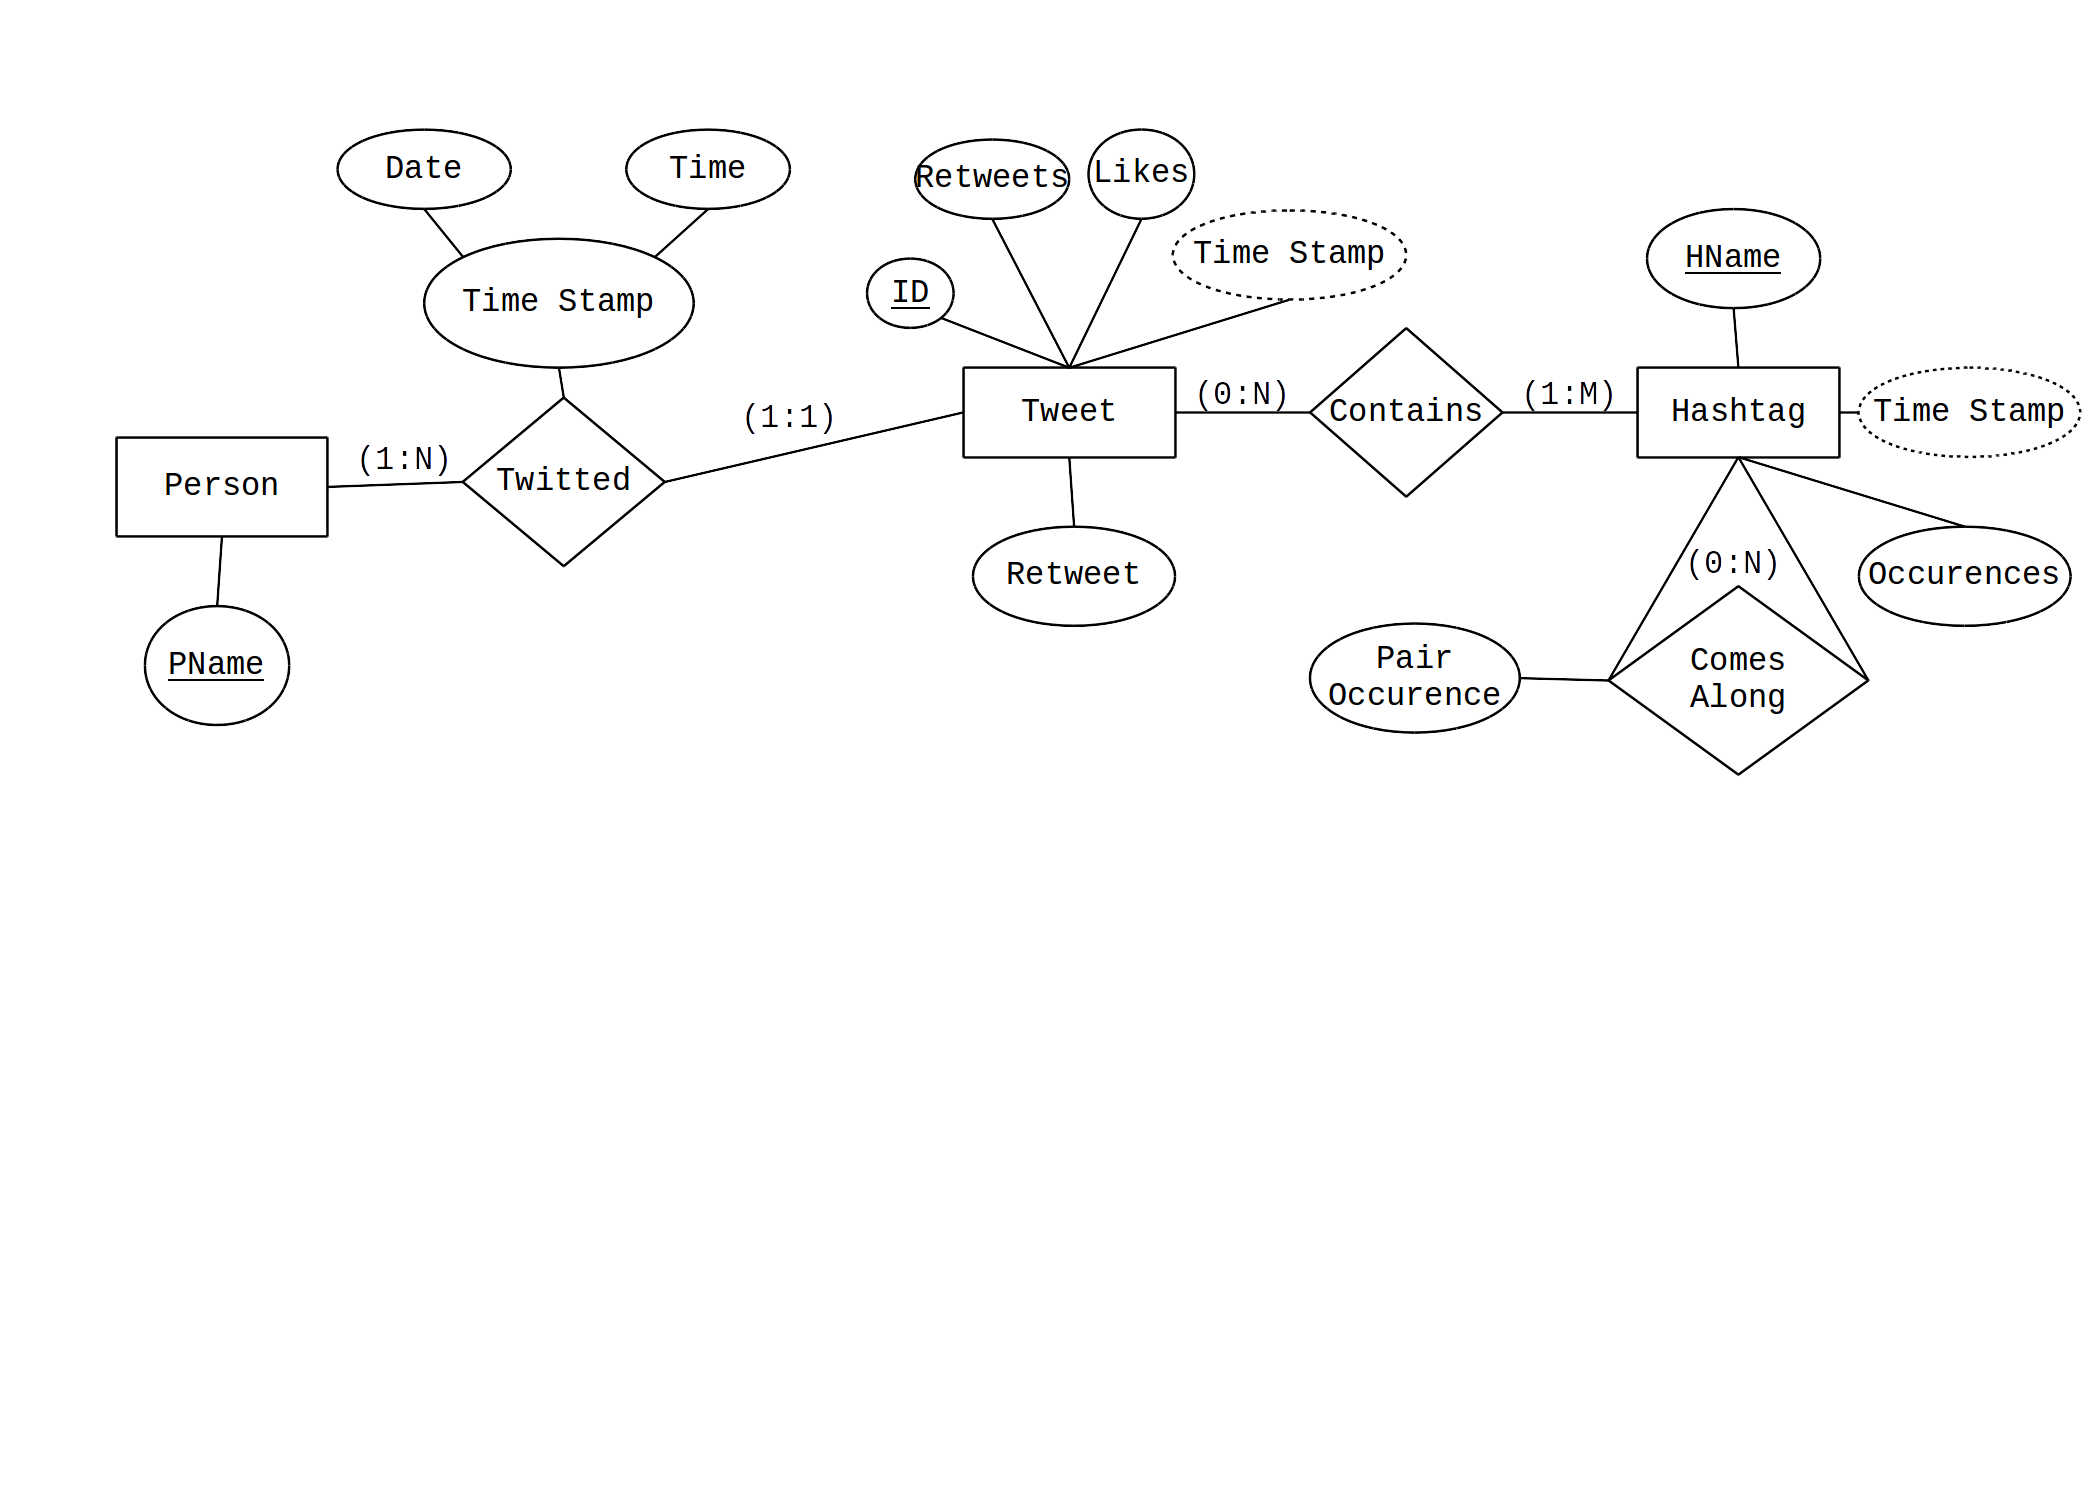
\includegraphics[scale=0.2]{MinMax_Diagram.png}
	\end{center}

	
	Im Zuge unserer Überlegungen hat sich unser Schema an mehreren Stellen vereinfachen lassen: das ursprüngliche modulare Modell hat sich zu einem monolithisch gerichteten Modell verändert. Beispielsweise haben wir erst \textit{Person} als Entität im ER-Diagramm dargestellt, haben aber im Nachhinein festgestellt, dass diese als Attribut der Entität \textit{Tweet} denselben Zweck erfüllt, ohne einen Umweg gehen zu müssen über die Relation \textit{Tweet} was \textit{Twitted} by \textit{Person}. Mehr dazu, ein Tweet kann jetzt mit dem Tupel (\textit{PName, Date, Time}) eindeutig identifiziert werden.
		
	\begin{center}
	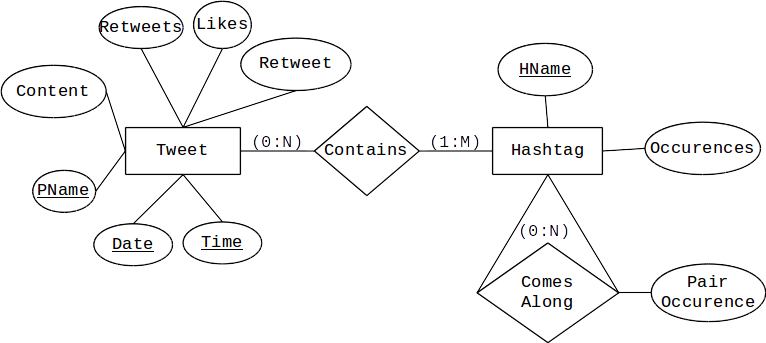
\includegraphics[scale=0.6]{MinMax_Diagram2}
	\end{center}
	
	Beschreibung des Diagramms:
	
	\begin{itemize}
	\item \textit{Tweet} - entspricht jeder Zeile in dem gegebenen Datensatz.
	\item \textit{Retweets, Likes} - Anzahl der Retweets und Likes von diesem Tweet. \textit{PName} ist der Autor des Tweets. Alle drei fassen das Superkey zusammen.
	\item \textit{Retweet} - Markiert, ob das Tweet ein Retweet ist.
	\item \textit{Content} - Der Inhalt des Tweets.
	\item \textit{Date, Time} - Die Datum und die Uhrzeit der Veröffentlichung eines Tweets, als zwei separate Attribute gespeichert, da die Informationen über die Long- bzw. Short-Term Entwicklung der Trends liefern können.
	\item \textit{Contains} - Diese Relation verbindet die Hashtags mit den Tweets, in denen sie Auftauchen.
	\item \textit{Hashtag} - Jeder Hashtag ist eine Entität.
	\item \textit{HName} - Name des Hastags, also der Hashtag selbst.
	\item \textit{Occurences} - Wie oft ein Hashtag auftaucht.
	\item \textit{Comes Along} - Diese Relation fasst zwei Hashtags als Paar zusammen. \textit{Pair Occurence} zählt wie oft ein Paar auftaucht.
	\end{itemize}

	Zusammenfassend ergibt sich das relationale Modell: \\

	Tweet(\underline{PName}, \underline{Date}, \underline{Time}, Retweets, Likes, Retweet, Content)\\
	Contains(\underline{Pname}, \underline{Date}, \underline{Time}, \underline{HName})\\
	Hashtag(\underline{HName}, Occurences)\\
	Comes Along(\underline{HName1}, \underline{HName2}, Pair Occurence)   
	
	\section{Datenbank erstellen}
	
	Die Datenbank zu erstellen ist relativ Einfach:
	\begin{enumerate}
	\item Shell-Login mit dem privilegierten Standard-PostgreSQL-Nutzer \texttt{postgres}, dann das \texttt{psql} Shell starten.
	\item Neues Nutzer erstellen (soll einem UNIX-Nutzer übereinstimmen) mit dem Befehl: \\ 
		\texttt{CREATE USER <UNIX-Nutzer> WITH PASSWORD '<password>';}
	\item Die Datenbank \textit{election} erstellen mit dem Befehl: \\
		\texttt{CREATE DATABASE election;}
	\item Letztens die Datenbank dem Nutzer zuweisen: \\
		\texttt{GRANT ALL PRIVILEGES ON DATABASE election to <UNIX-Nutzer>;}
	\end{enumerate}
	Der Nutzer hat jetzt Zugriff auf die Datenbank \textit{election} mit \texttt{psql} indem er in einem Terminal das Folgende aufruft: \\
	\texttt{\$ psql -d election}

\end{document}
